%%%Variables

%%%
\question[10] A ball moves through the air following the path described in the figure below \\
\begin{tabular}{cc}
	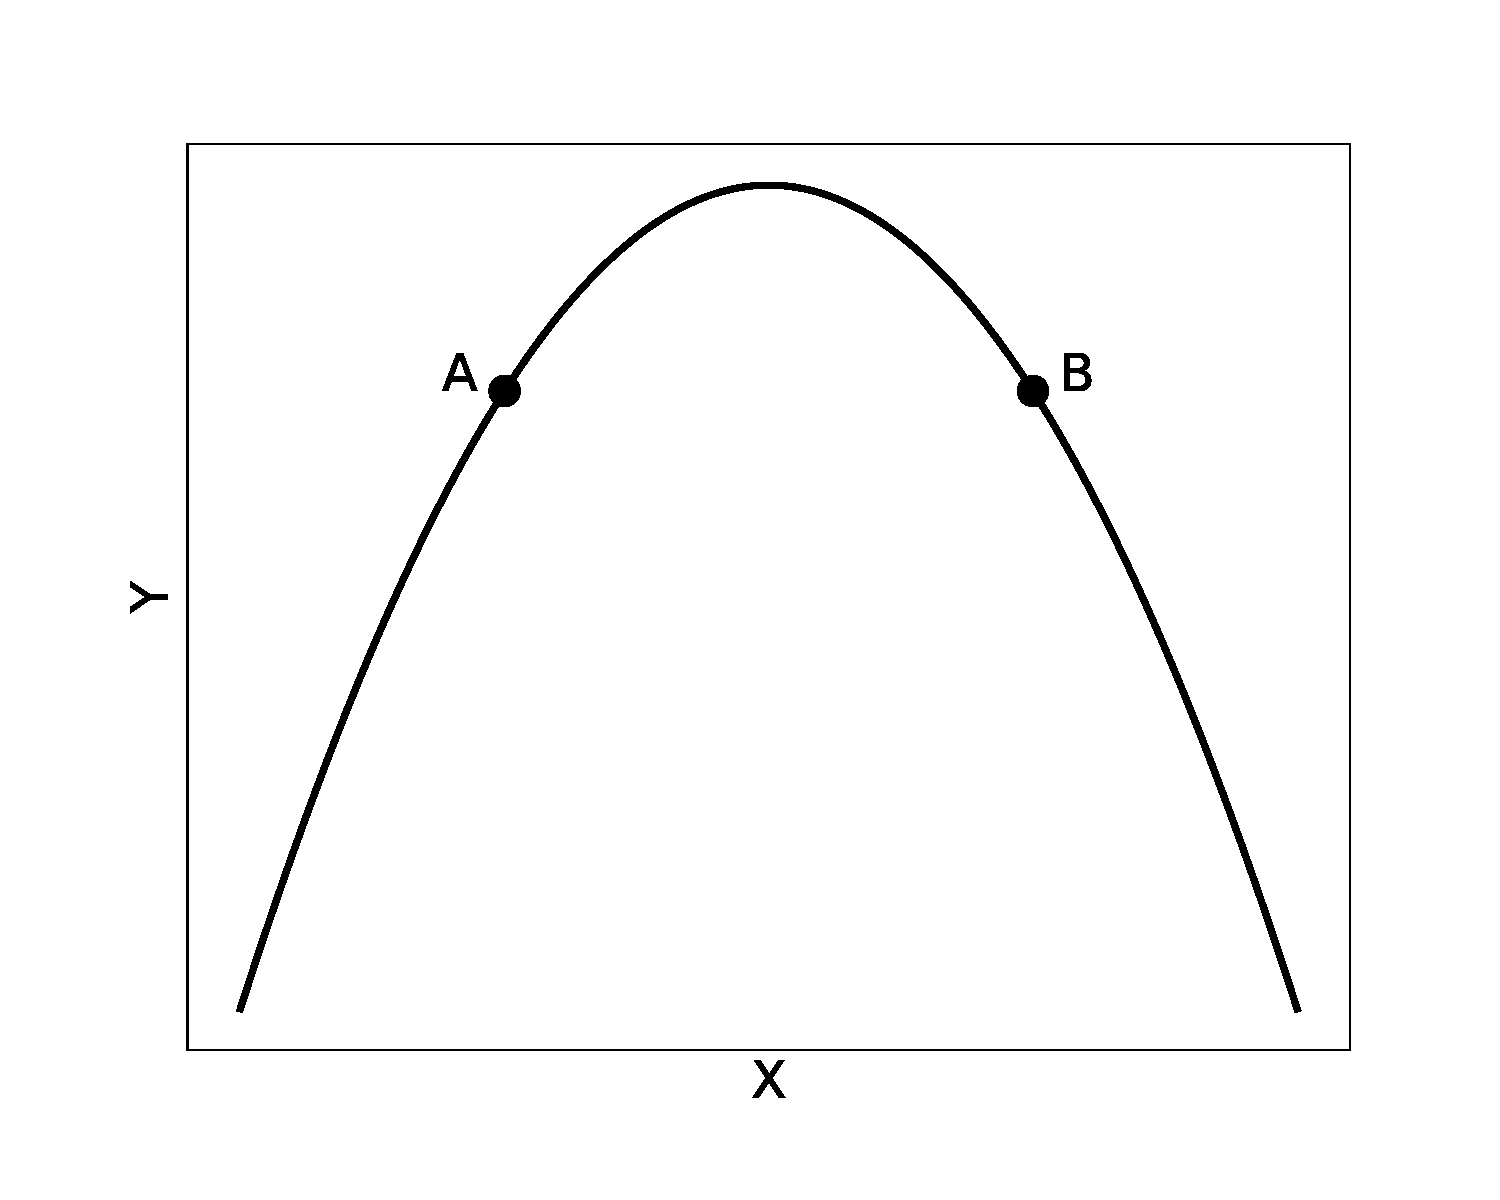
\includegraphics[width=10cm]{avg_velocity_fig.pdf} & 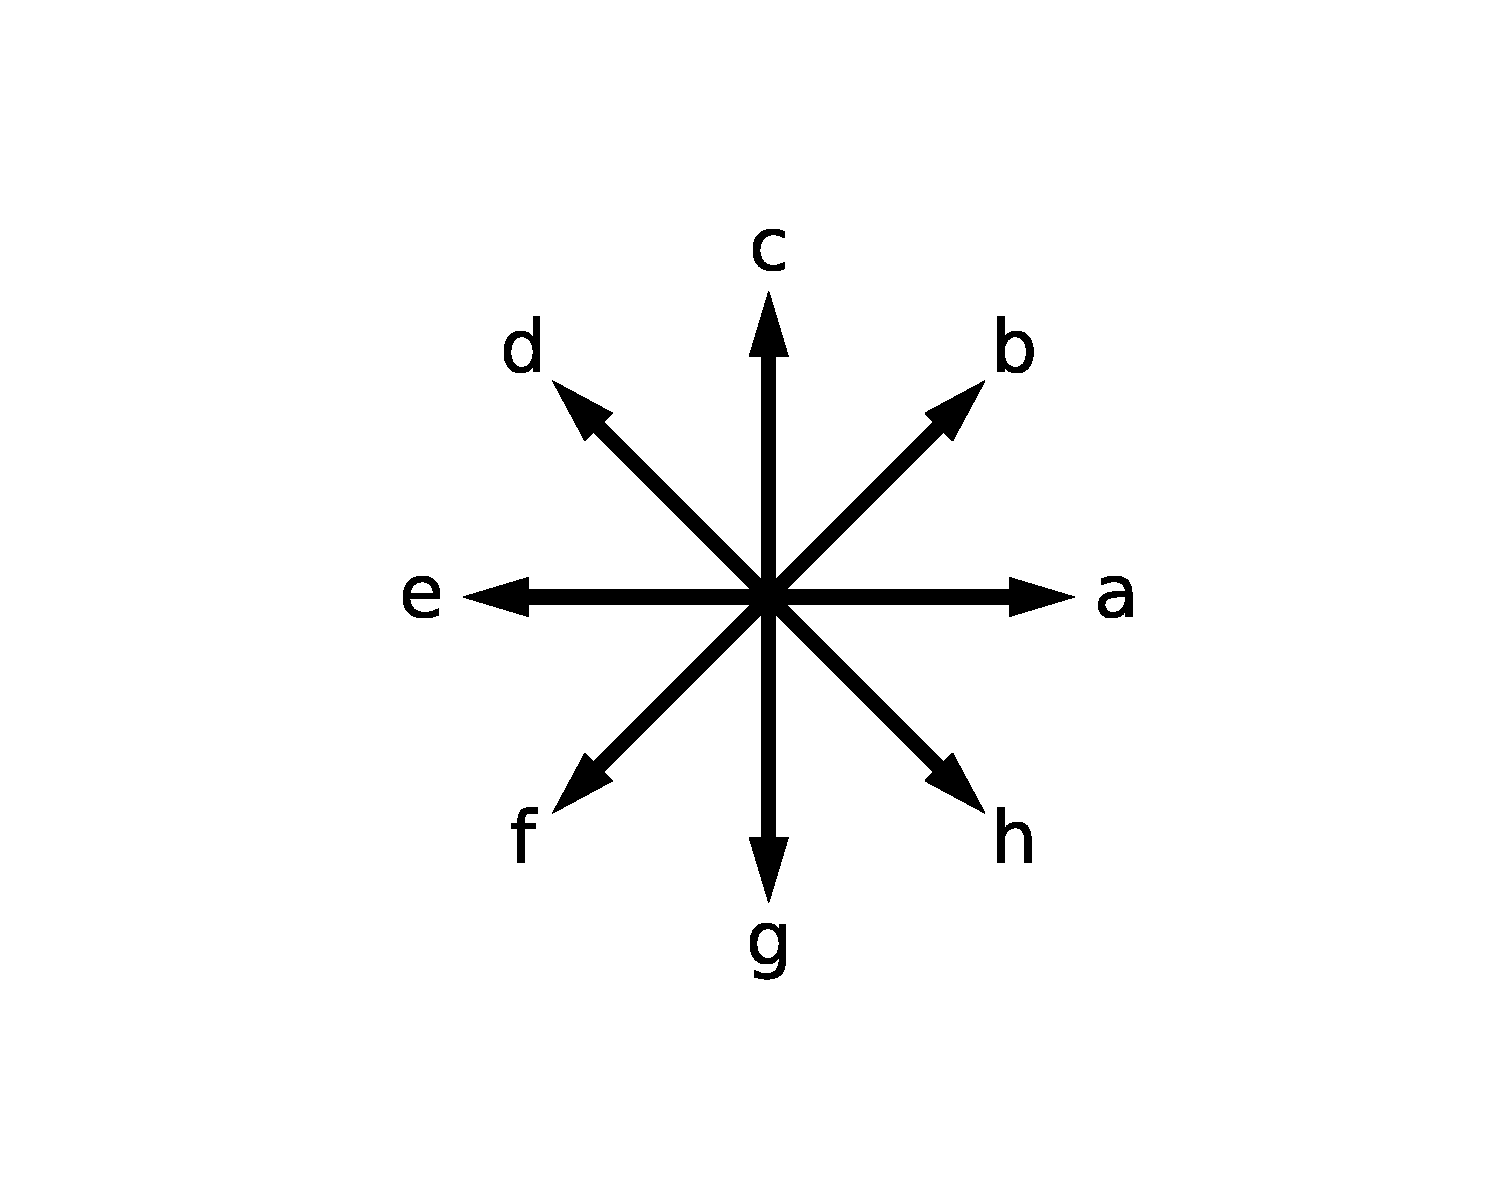
\includegraphics[width=8cm]{arrow_choices.pdf}
\end{tabular}
\begin{parts}
\part Which arrow (a-h) best describes the direction of the ball's average velocity from point $A$ to point $B$?\\
\begin{oneparcheckboxes}
	\choice a
	\choice b
	\choice c
	\choice d
	\choice e
	\choice f
	\choice g
	\choice h
\end{oneparcheckboxes}
	
\part Which arrow (a-h) best describes the direction of the ball's instantaneous velocity at point $B$?\\
\begin{oneparcheckboxes}
	\choice a
	\choice b
	\choice c
	\choice d
	\choice e
	\choice f
	\choice g
	\choice h
\end{oneparcheckboxes}

\part Which arrow (a-h) best describes the direction of the ball's instantaneous momentum at point $A$?\\
\begin{oneparcheckboxes}
	\choice a
	\choice b
	\choice c
	\choice d
	\choice e
	\choice f
	\choice g
	\choice h
\end{oneparcheckboxes}
\part Which arrow (a-h) best describes the direction of the change in the ball's momentum from point $A$ to point $B$?\\
\begin{oneparcheckboxes}
	\choice a
	\choice b
	\choice c
	\choice d
	\choice e
	\choice f
	\choice g
	\choice h
\end{oneparcheckboxes}
\part Is the ball experiencing an interaction with another object? Explain.
\end{parts}